\chapter{战场的两面：日本人墓地与英联邦战争公墓}

\section{两处墓地，一座小岛}

新加坡是一座极小的岛屿，却在方寸之地上，同时安葬着一场战争的两面。

一边是日本人墓地公园，静默于城市一隅，杂草与三角梅交织，石碑风化，岁月斑驳；另一边是克兰芝战争纪念公园，由英联邦战争墓地委员会出资维护，草坪整洁，白色墓碑成排伫立，庄严肃穆。

前者埋葬的，是侵略者，以及那些被历史遗忘的女人。后者埋葬的，是被侵略者，以及那场沦陷的记忆。

\section{日本人墓地公园：被时间遗忘的地方}

日本人墓地公园位于新加坡东北部的后港（Hougang），地址为 22 Chuan Hoe Ave。这片占地约 29,000 平方米的墓地，是东南亚规模最大的日本人墓地，共有 910 块墓碑。1969 年，新加坡政府将墓地的所有权移交给\textbf{日本人协会（Japanese Association of Singapore）}，由其负责日常维护至今；1987 年，该地被正式指定为纪念公园。

走进日本人墓地公园，第一个感受是安静。

不是那种肃穆的安静，而是一种被遗忘的安静。墓地里的石碑大多低矮简朴，表面布满苔藓，有些已经倾斜，有些已经破损。紫红色的三角梅从旁边攀爬过来，覆在几座石碑之上——花朵盛开，颜色鲜艳，与灰色的石碑形成一种奇异的对比。生命与死亡，在这里以一种意想不到的方式并置。

\begin{figure}[h]
\centering
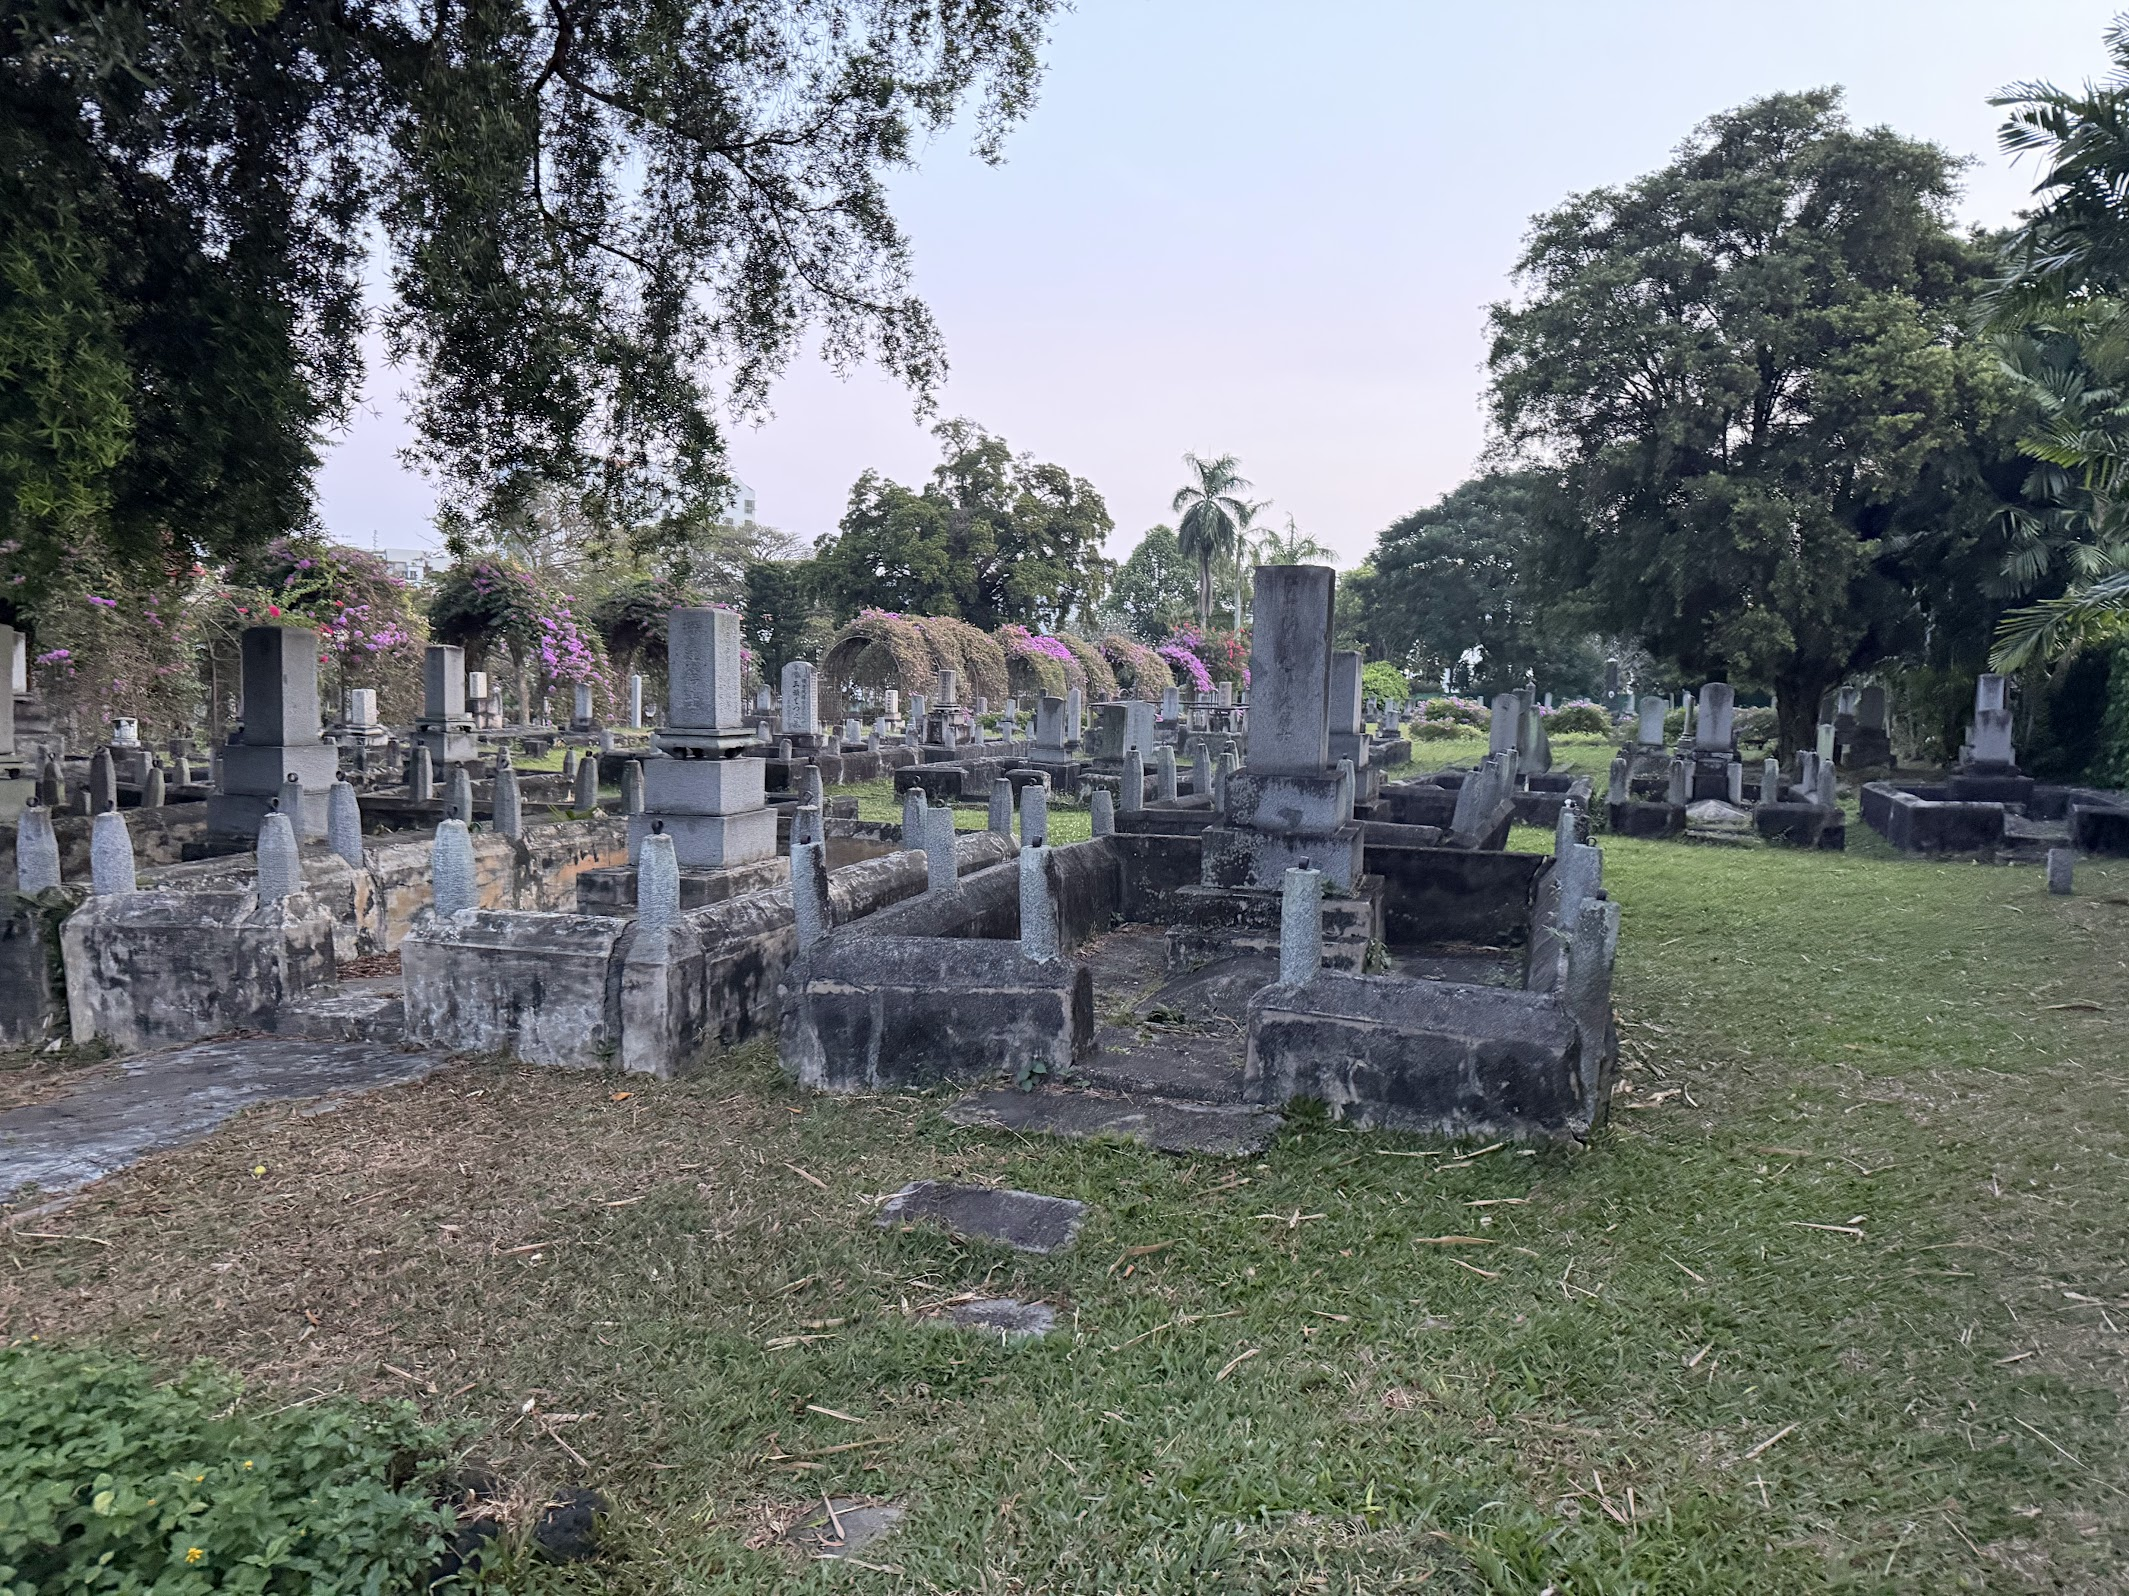
\includegraphics[width=0.8\textwidth]{../../pictures/japanese tomb/IMG_9019}
\caption{三角梅攀爬在风化的墓碑之上}
\end{figure}

开阔的草地上，数十座墓碑散落其间，间距不均，排列随意，没有任何刻意的秩序感。清晨或黄昏的柔光打下来，整片墓地显得格外空旷。

\begin{figure}[h]
\centering
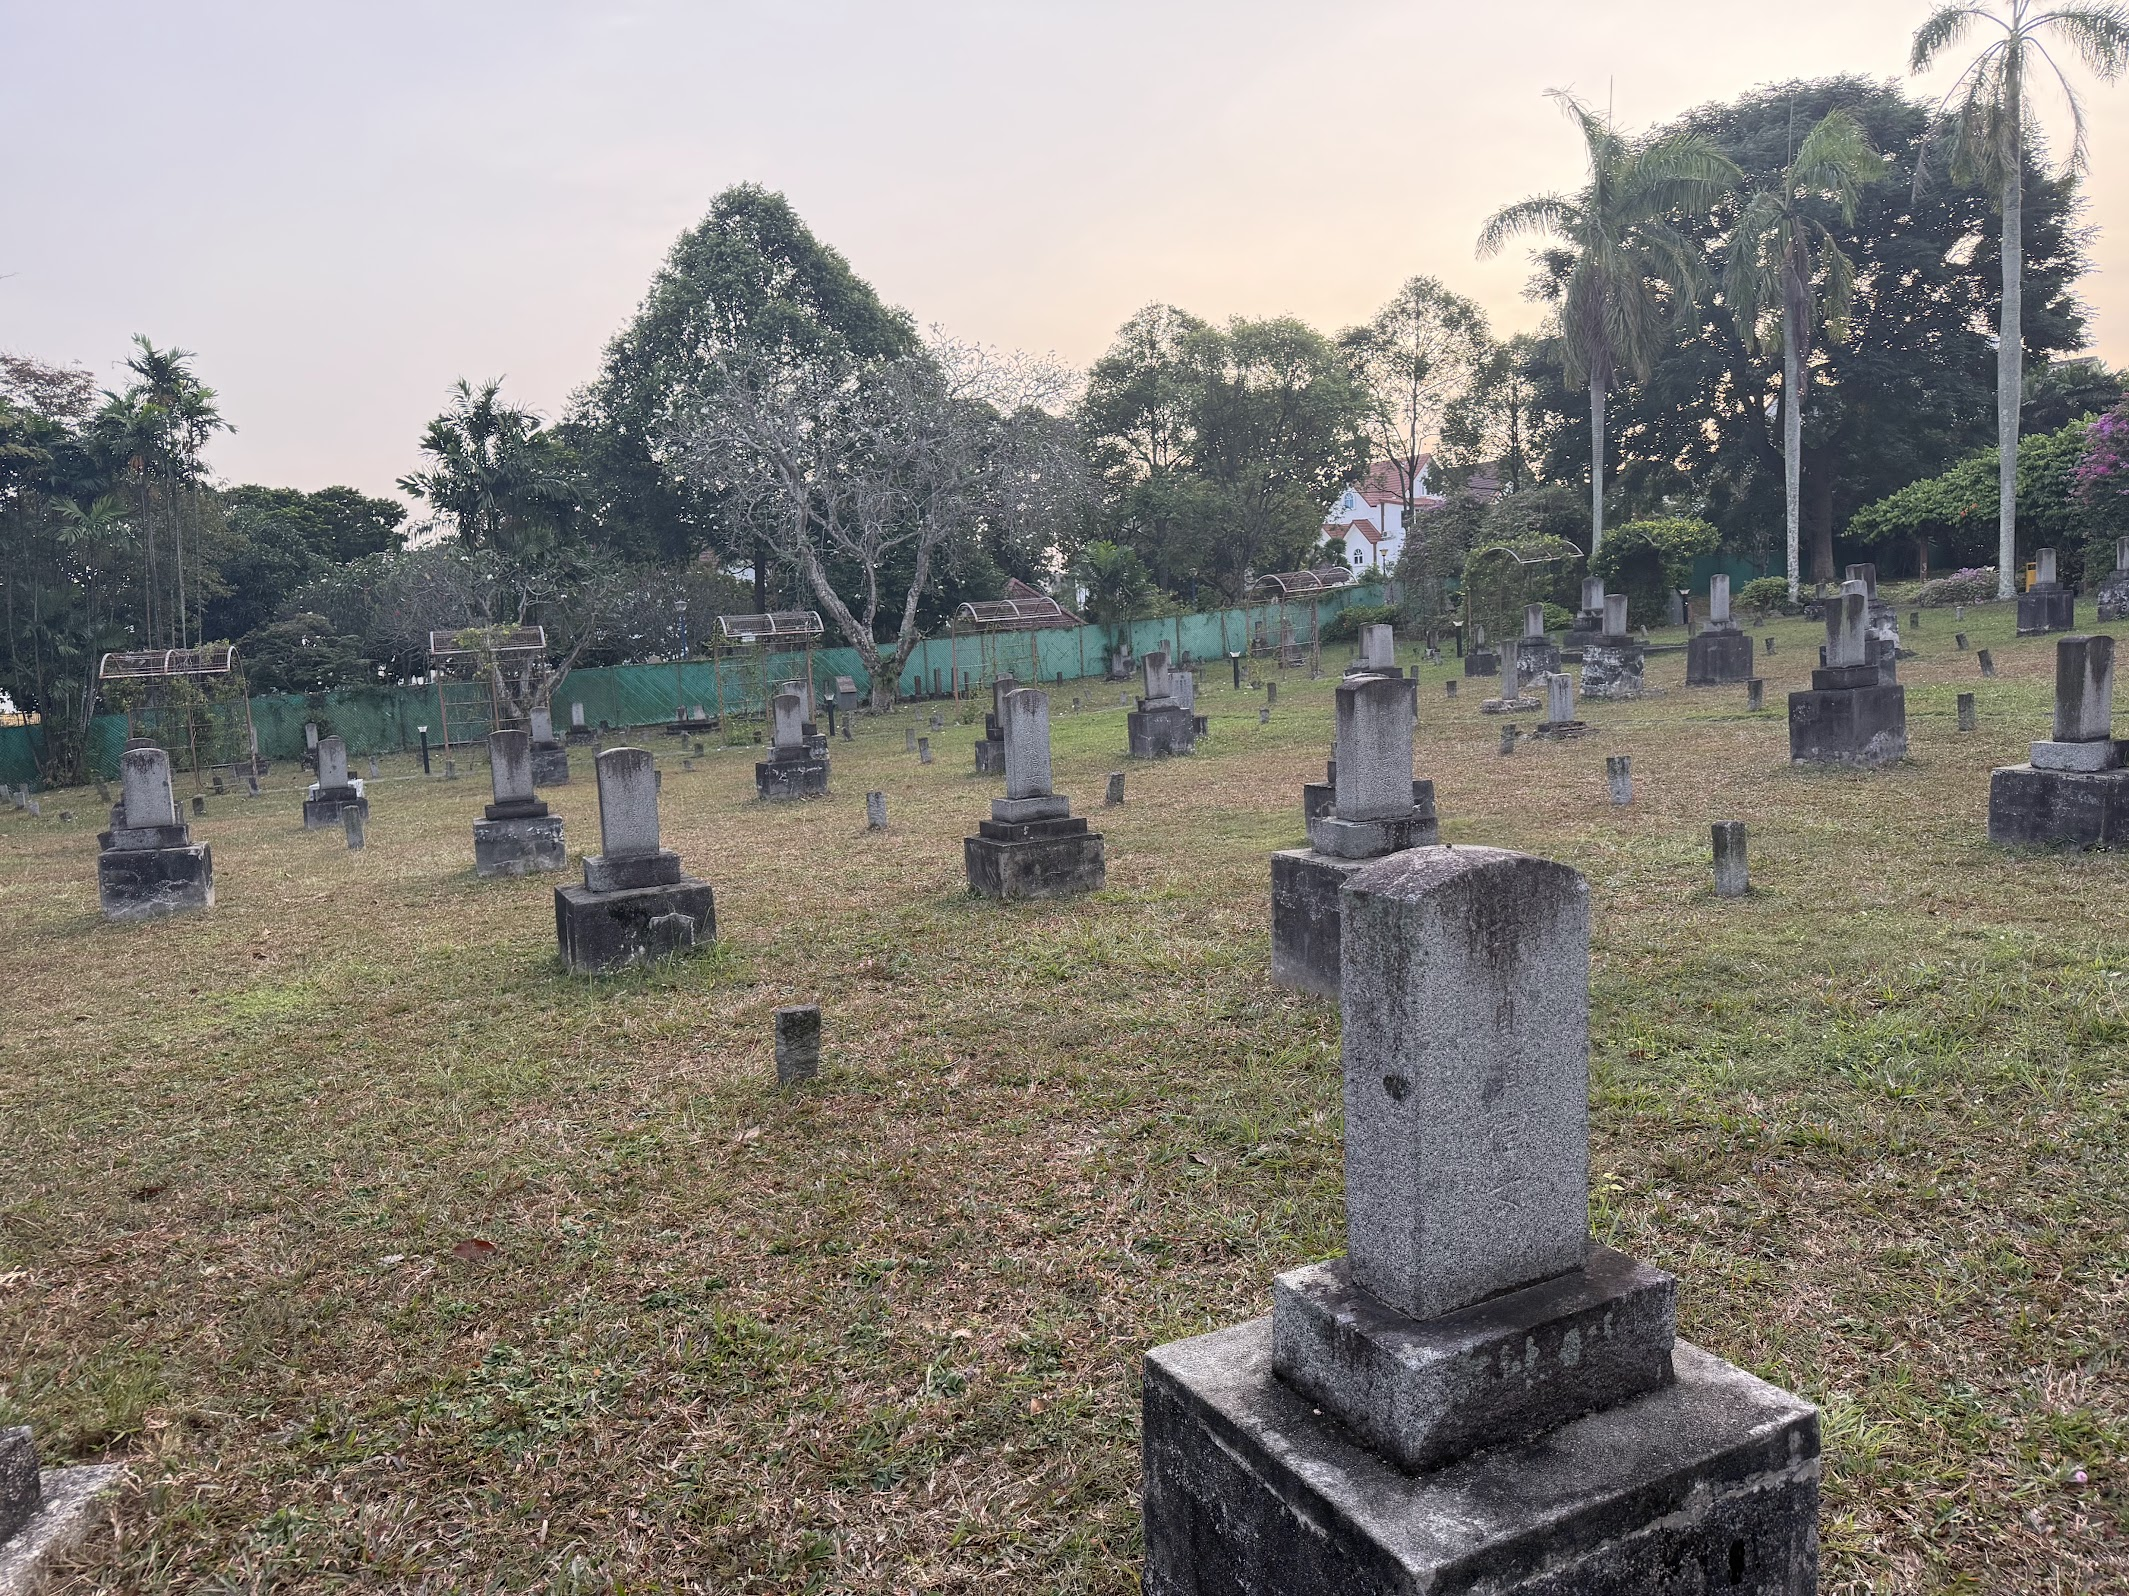
\includegraphics[width=0.8\textwidth]{../../pictures/japanese tomb/IMG_9080}
\caption{墓地全景：草地上散落的低矮石碑}
\end{figure}

\section{先进墓地：七十七位被命名的女人}

在墓地的一角，有一块说明牌，标题写着"先進墓地（ぱいおにあ）"——先进墓地，Pioneer Cemetery。

说明牌介绍了一位名叫 \textbf{Toma Sato} 的女性，卒于 1899 年。她是一位 \textbf{karayuki-san（唐行さん）}——19 世纪末至 20 世纪初，大批日本女性漂洋过海来到东南亚，其中许多人从事性工作。她们被称为"唐行さん"，意为"去了唐山（中国）的人"，但实际上足迹遍布整个东南亚。

说明牌上记载：这片围墙之内，共有 \textbf{77 座墓}，全部属于 karayuki-san，卒年介于 \textbf{1899 年至 1938 年}之间。这块墓地曾被英国殖民政府用作土地边界标记——她们死后，连身体也成了殖民地图上的一个坐标。

\begin{figure}[h]
\centering
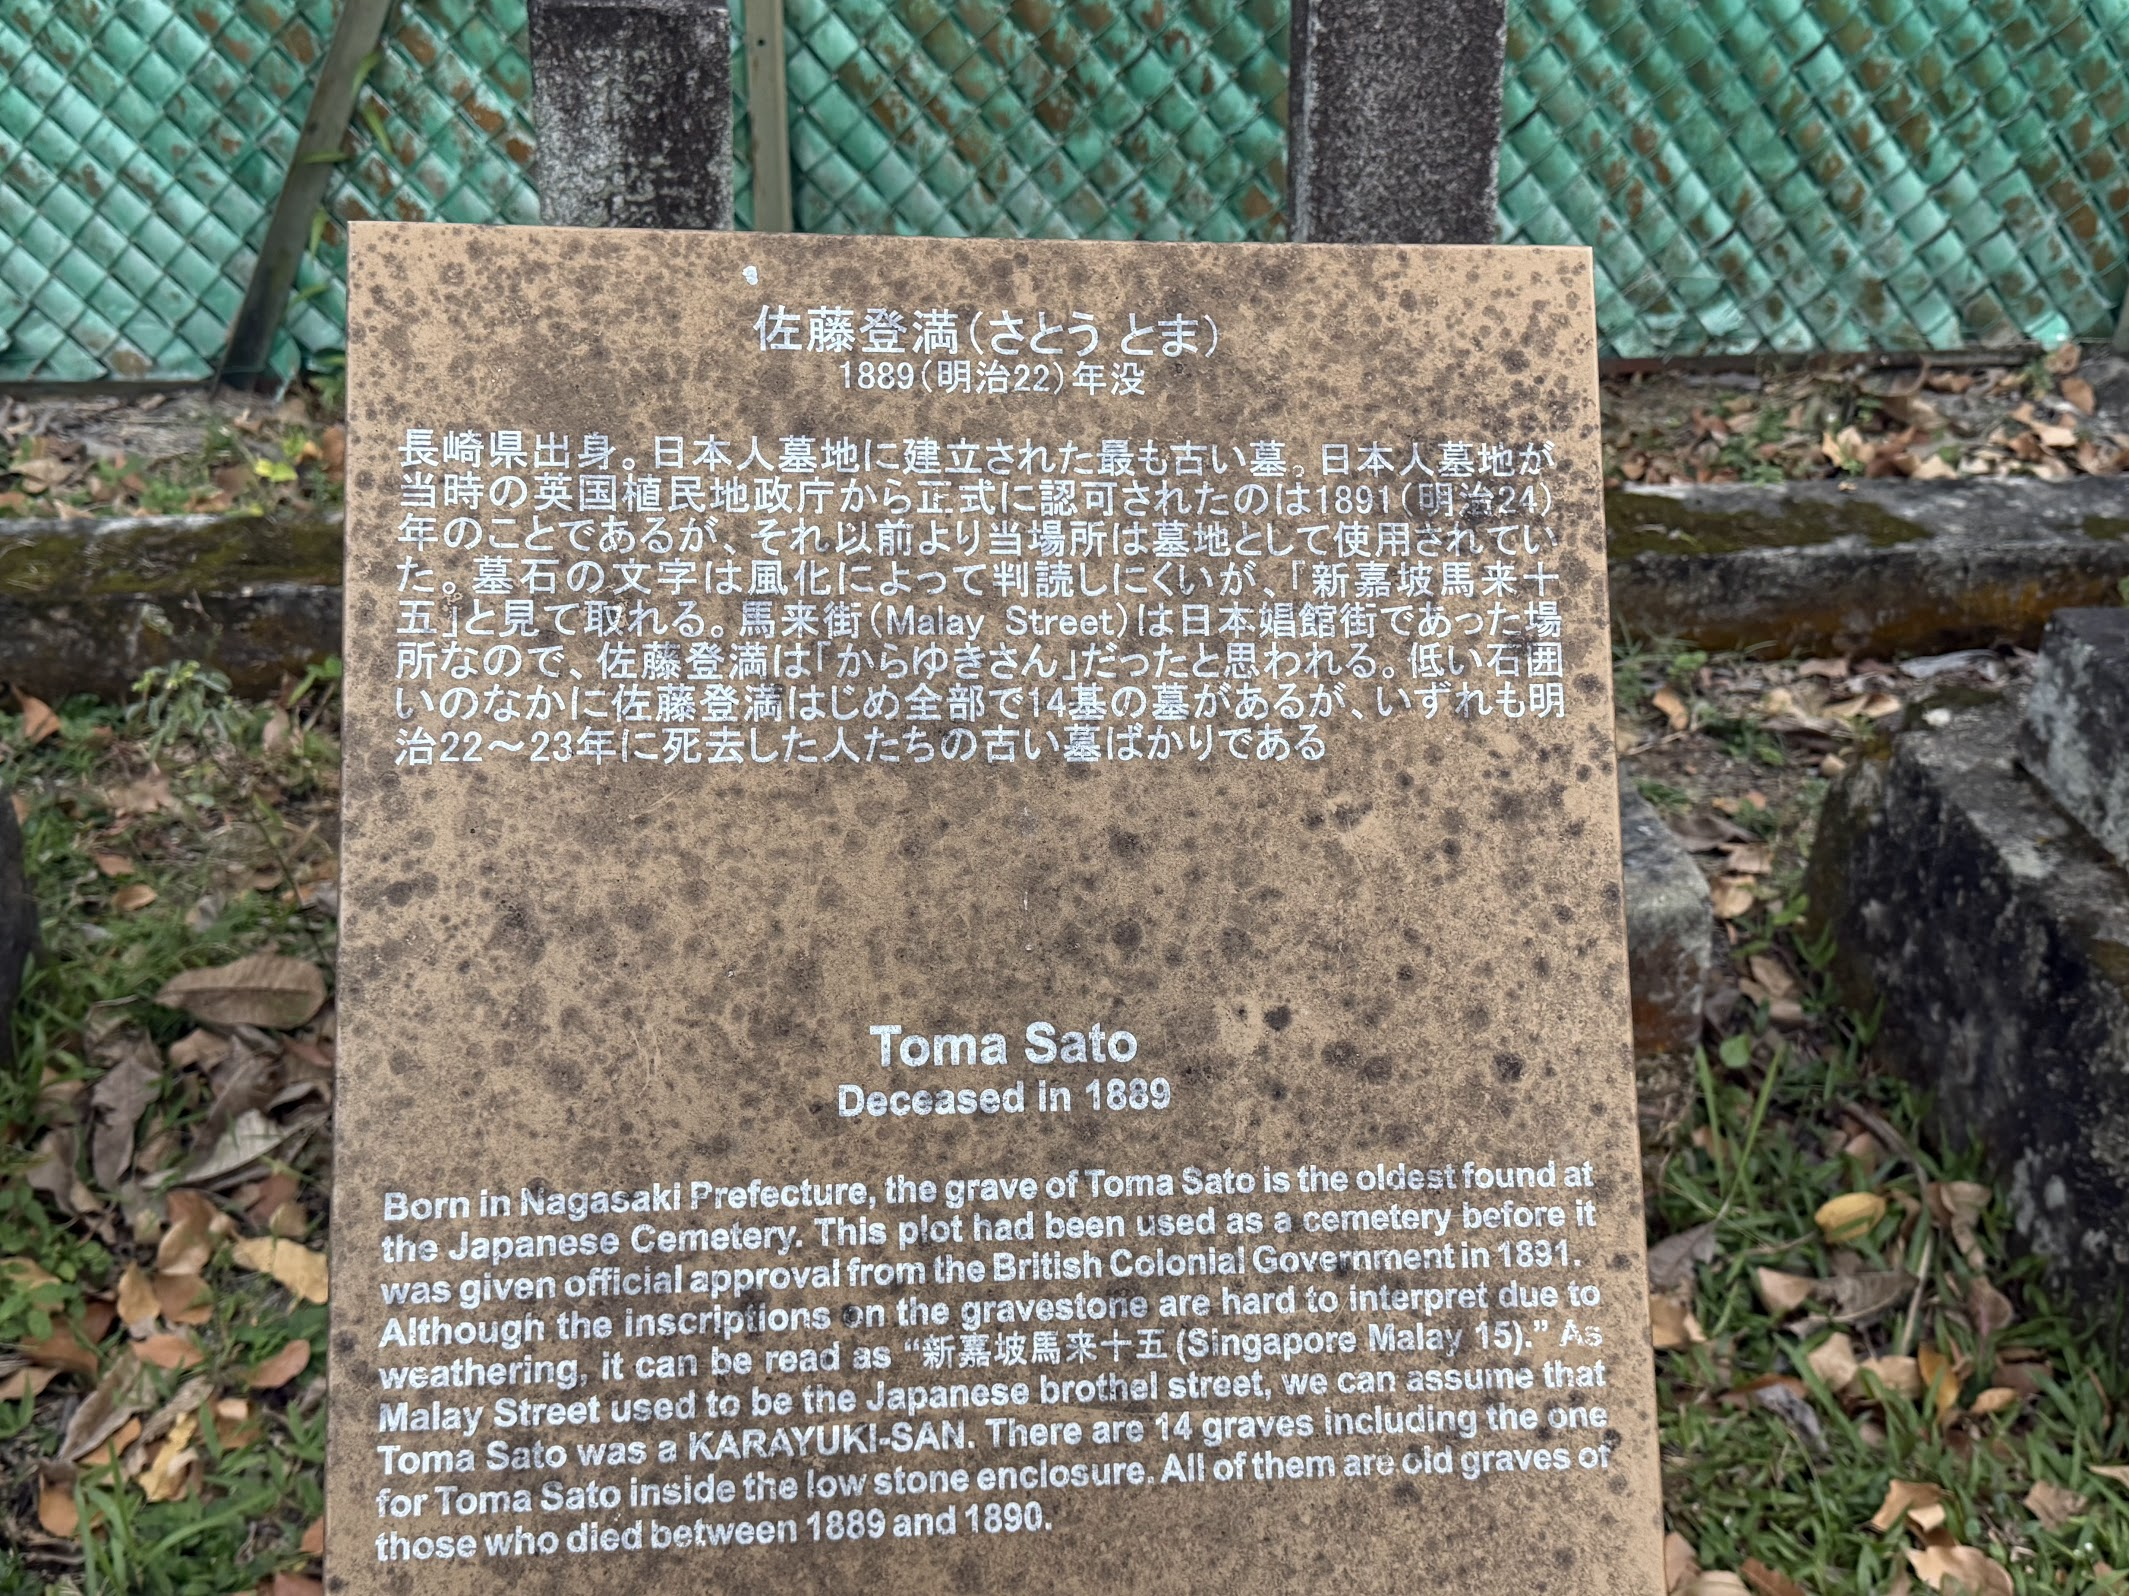
\includegraphics[width=0.8\textwidth]{../../pictures/japanese tomb/IMG_9048}
\caption{先进墓地说明牌，介绍 Toma Sato 与 77 位 karayuki-san}
\end{figure}

新加坡官方在此竖立说明牌，以中英日三语正式标注"KARAYUKI-SAN"，这本身已是一种历史的承认。然而，承认之后呢？

\section{仍有人记得}

在另一处，一座保存相对完好的日式石碑独立而立，碑身刻有日文字符，碑前摆着香炉和供品台。香灰尚新，说明不久前有人来过。

在这片大多已被遗忘的墓地里，这座碑显得格外珍贵。有人记得。不知是后裔，还是某个默默守护这段历史的人。

\begin{figure}[h]
\centering
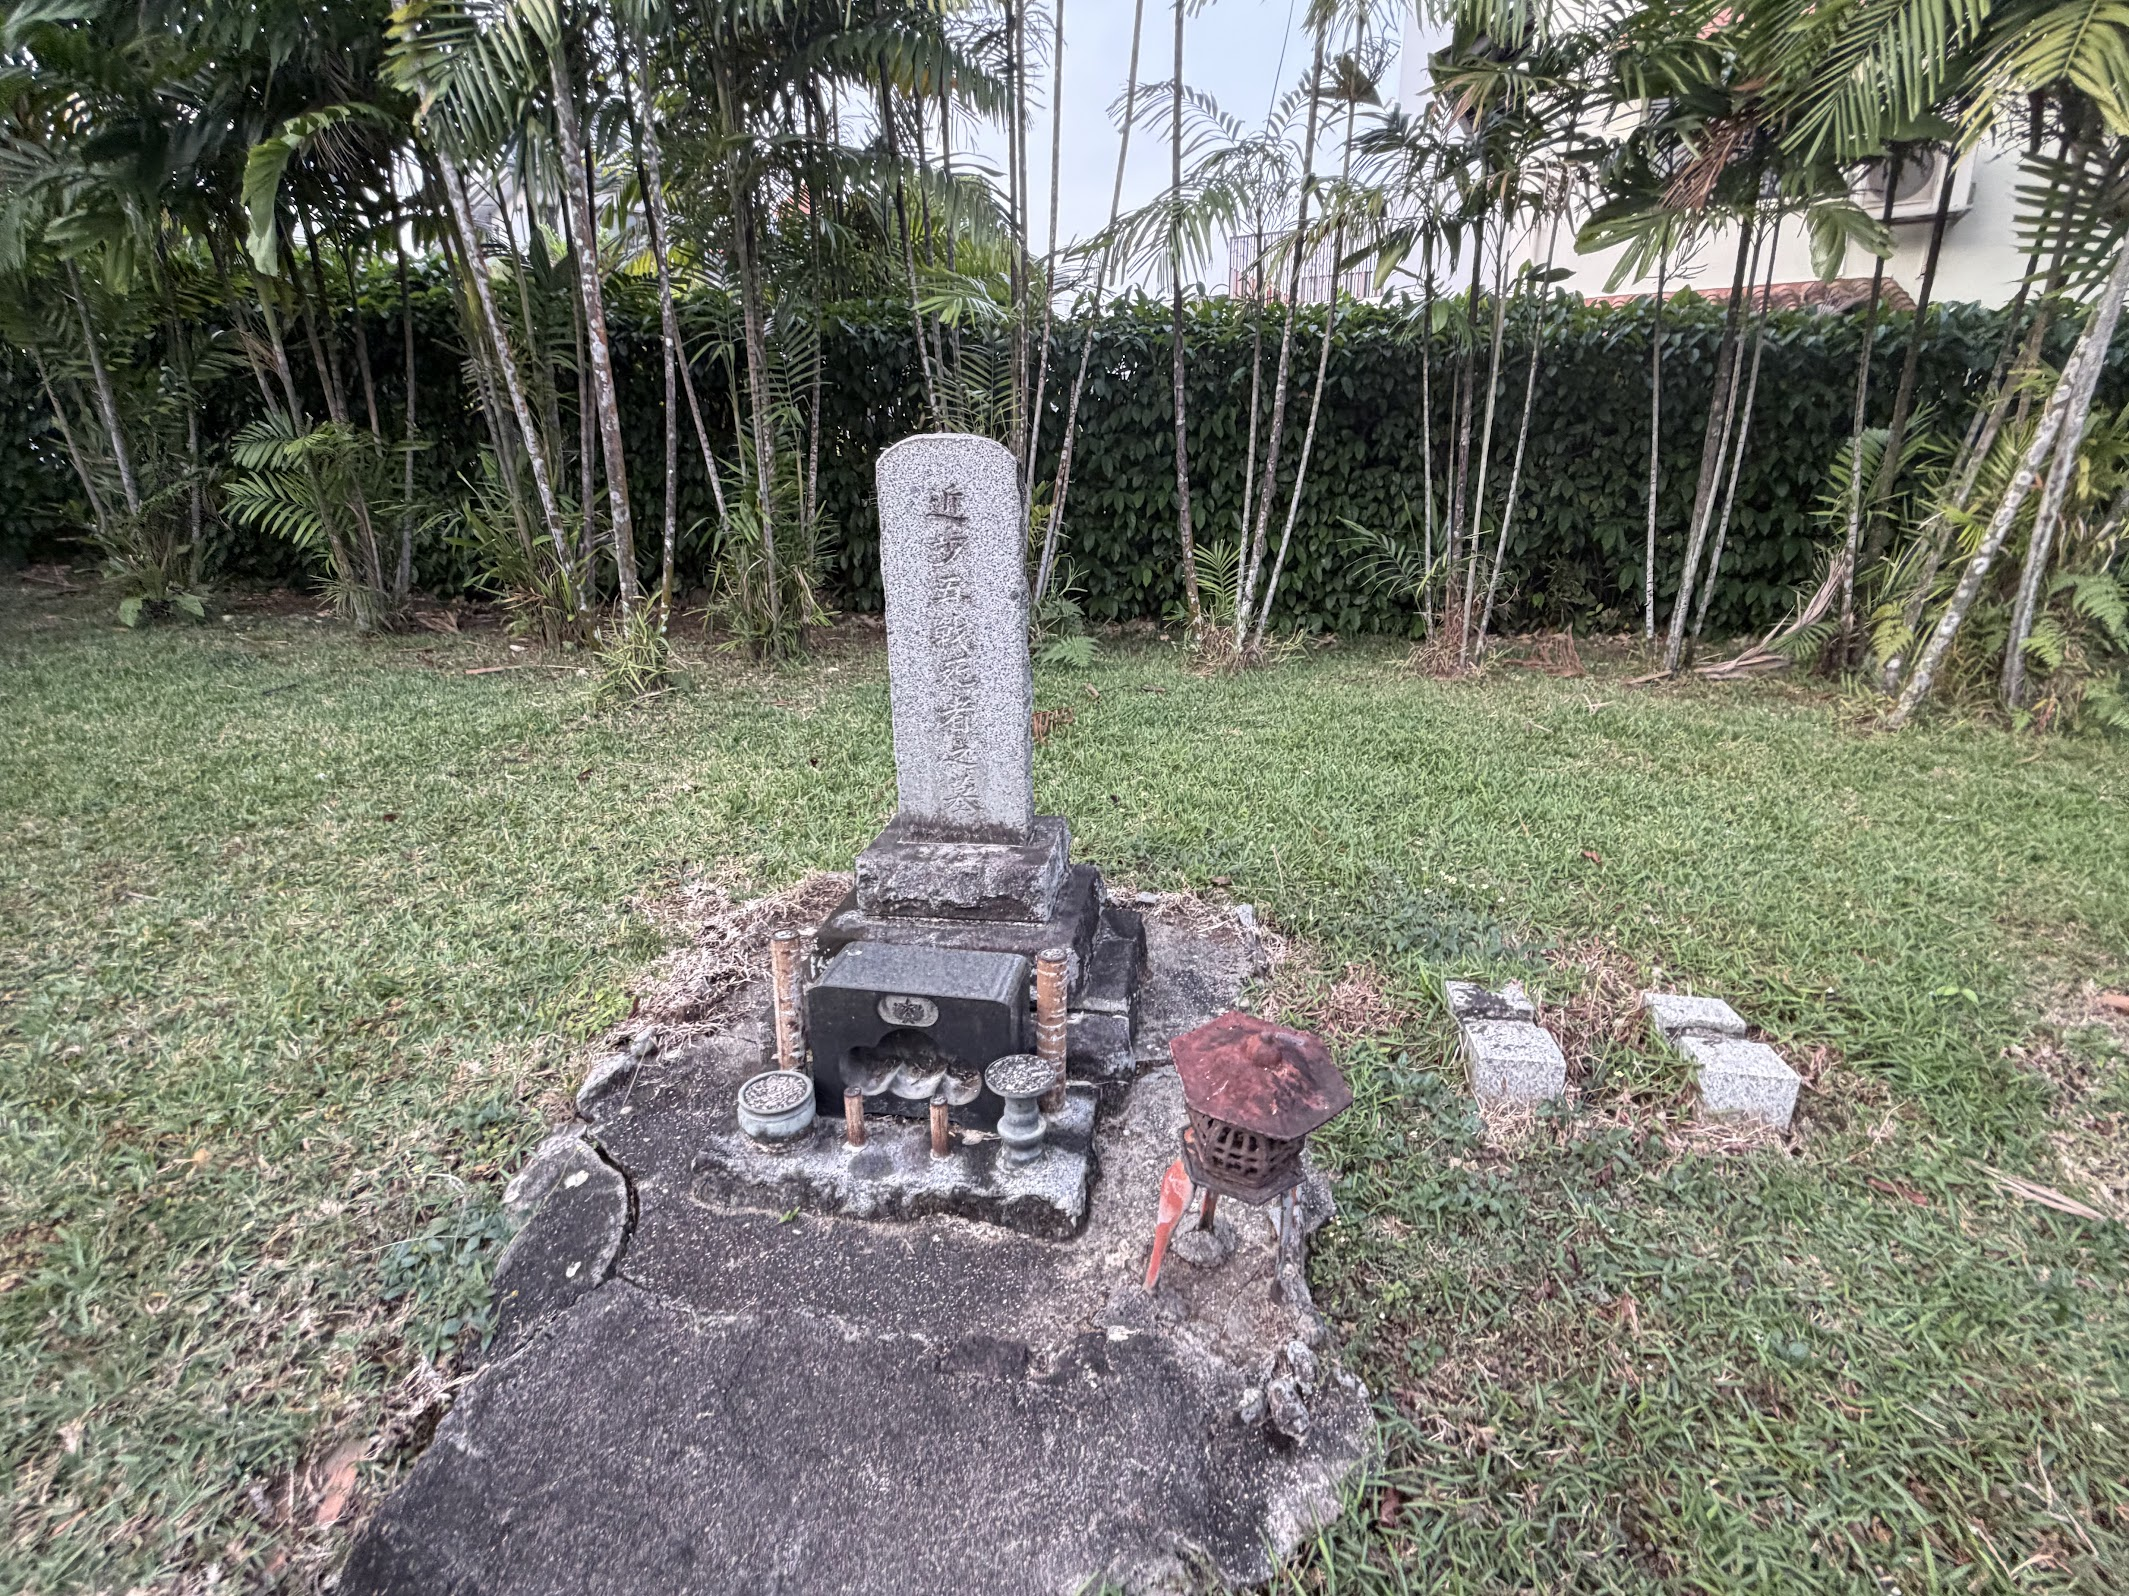
\includegraphics[width=0.8\textwidth]{../../pictures/japanese tomb/IMG_9124}
\caption{仍有人祭扫的石碑，碑前摆有香炉与供品}
\end{figure}

墓地的另一侧，摆放着几张石质长椅，石板小径蜿蜒其间。这里的氛围，已不完全像一座墓地，更像一座公园。新加坡对这片土地的定位，是双重的：纪念之地，也是市民休憩的公共绿地。

\begin{figure}[h]
\centering
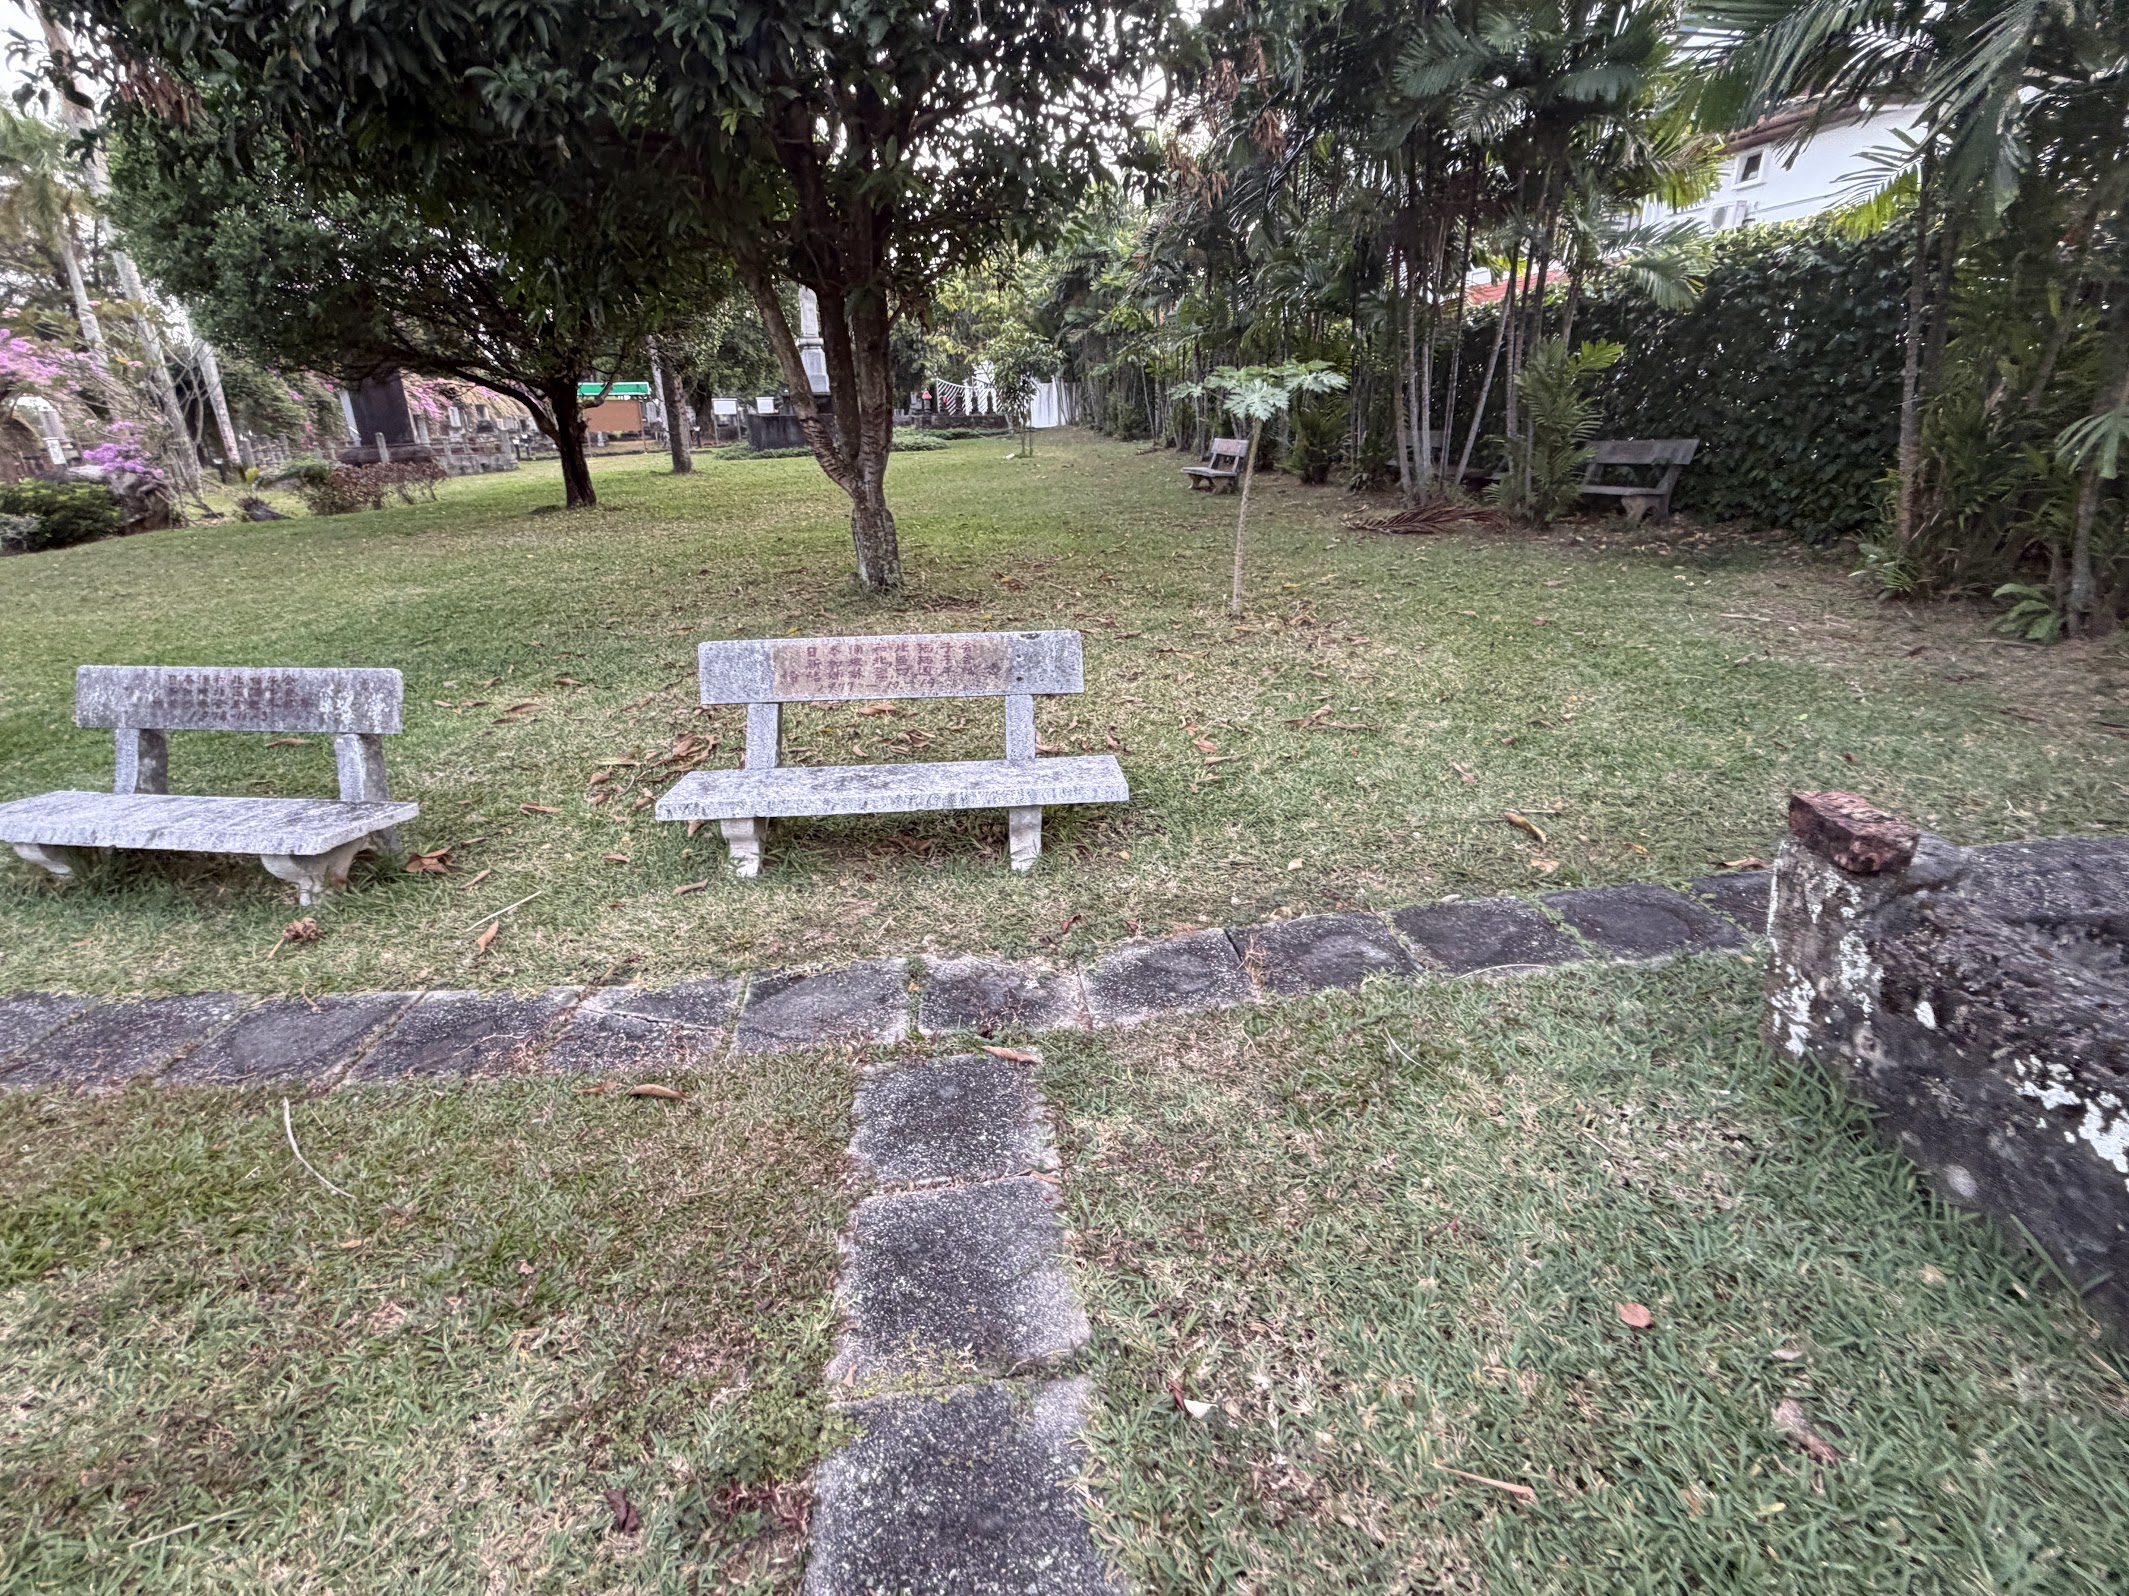
\includegraphics[width=0.8\textwidth]{../../pictures/japanese tomb/IMG_9129}
\caption{石质长椅与蜿蜒小径，氛围更像公园}
\end{figure}

这种双重性，令人沉思。公园化的处理，是一种包容，还是一种温和的遗忘？

\section{克兰芝：另一种记忆的方式}

与日本人墓地公园的荒疏相比，克兰芝战争纪念公园是另一个世界。

克兰芝战争公墓（Kranji War Cemetery）位于新加坡北部，地址为 9 Woodlands Road，坐落于新加坡岛的北岸高地之上，俯瞰柔佛海峡（Straits of Johore），隔水遥望马来西亚。这一地理位置并非偶然——1942 年 2 月 8 日，日军正是从这片海峡渡海，在克兰芝河口附近登陆，距今日公墓所在地不足三公里。

率领这场攻势的，是日本第 25 军司令官山下奉文（Yamashita Tomoyuki）。他指挥的日军在进攻新加坡之前，已沿马来半岛一路南下，以自行车代马，骑行穿越丛林与公路，仅用约 70 天便从泰国南部打到了新加坡北岸。这场"自行车闪击战（Bicycle Blitzkrieg）"令英军猝不及防，山下奉文也因此赢得了"\textbf{马来之虎}（Tiger of Malaya）"的称号。英军的重炮原本朝向南方大海，防范的是从海上来袭的敌人——却没想到，敌人骑着自行车从背后杀来。

这里由英联邦战争墓地委员会（Commonwealth War Graves Commission，CWGC）出资维护，长期保持整洁。白色墓碑整齐排列，草坪修剪精细，庄严而克制。这里安葬的，是 1942 年新加坡沦陷（Fall of Singapore）期间牺牲的盟军士兵——英国、澳大利亚、印度、马来亚等地的军人，以及其他为抵抗日军而牺牲的人。

每一块墓碑上都刻着名字、军衔、日期。没有无名之墓。

这种记忆方式，是有组织、有资金、有制度保障的。胜利者的记忆，往往比失败者的更持久，也更整齐。

\section{谁被记住，谁被遗忘}

站在这两处墓地之间，我反复想着同一个问题：谁被记住，谁被遗忘？

克兰芝的士兵们，有名字，有国家，有委员会为他们除草、立碑、维护档案。而日本人墓地里的 77 位 karayuki-san，在历史上几乎默默无闻，直到一块说明牌的出现，才让她们的存在得以被路过的人看见。

她们不是战士，不是英雄，甚至在自己的国家也是被羞耻所笼罩的存在。但她们同样死在这座岛上，同样被热带的泥土所收纳。

新加坡今天与日本关系友好，经济往来密切。这段战争的历史，既没有被大张旗鼓地清算，也没有被彻底抹去。日本人墓地依然存在，说明牌依然竖立。这，也许就是新加坡处理历史的方式：保留，但不放大；承认，但不纠缠。

在刀锋上生存的小国，没有太多余裕用于仇恨。
